\documentclass[conference]{IEEEtran}

\usepackage{amsmath,amssymb,amsfonts}
\usepackage{booktabs}
\usepackage{cite}
\usepackage{graphicx}
\usepackage{textcomp}
\usepackage{xcolor}
\usepackage{url}
\usepackage{xspace}
\usepackage[section]{placeins}

\graphicspath{{assets/paper/}}

\newcommand{\modelname}{Simamba\xspace}
\newcommand{\mamba}{Mamba\xspace}
\newcommand{\mambatwo}{Mamba--2\xspace}
\newcommand{\mambathree}{Mamba--3\xspace}

\begin{document}

\title{\modelname: Evaluating Simpson-Style Discretization for Mamba--3 State Space Language Models}

\author{
\IEEEauthorblockN{Soumil Baldota, Ansen Shia, and David Zhang}
\IEEEauthorblockA{
\textit{School of Engineering and Applied Sciences}\\
\textit{Columbia University}\\
New York, NY, USA\\
\{ssb2234, as8008, dwz2107\}@columbia.edu
}
}

\maketitle

\begin{abstract}
State space sequence models offer linear-time alternatives to Transformer attention, but their quality and stability depend strongly on the numerical discretization used to update recurrent state. This project studies whether a Simpson-style update can improve the single-input single-output (SISO) recurrence used in \mambathree. We implement \modelname, a \mambathree-inspired mixer that replaces the matched trapezoid state update with a learned width-3 Simpson recurrence, and we build the end-to-end training, evaluation, checkpointing, benchmarking, and Hugging Face/vLLM export pipeline needed to test it. On a single Tesla V100, we train controlled 10M-parameter language models on SlimPajama subsets with fixed validation sampling, no-replacement training sampling, AdamW, cosine learning-rate decay, fp32 parameter storage, and gradient health logging. The final controlled runs are stable, but the current Simpson parameterization does not outperform the baselines: on the 500M-token experiment, \mambatwo reaches validation loss 4.8625, the best \modelname Simpson-midpoint run reaches 4.9178, and the matched \modelname trapezoid run reaches 4.9326. At the 50M-token budget, trapezoid remains ahead of Simpson both without local convolution (5.8195 vs. 5.8929--5.9178) and with matched causal local mixing (5.8469 vs. 5.8793--5.8890). The systems result is similarly mixed: decode-step latency is within about 8\% of \mambathree in the repository benchmark, but current \modelname prefill is hundreds of times slower and requires fused-kernel work. The main contribution is therefore a reproducible negative result and a diagnosis: Simpson's negative lag-2 correction is mathematically plausible but currently harder to optimize than the trapezoid update.
\end{abstract}

\begin{IEEEkeywords}
state space models, Mamba, language modeling, discretization, Simpson's rule, vLLM, GPU training
\end{IEEEkeywords}

\section{Introduction}

Selective state space models (SSMs), especially the \mamba family, have become a practical alternative to attention for sequence modeling because they replace quadratic all-pairs attention with linear-time recurrent scans while preserving strong language-modeling quality \cite{mamba,mamba2}. The latest \mambathree line extends this direction with inference-first SISO state dynamics and specialized kernels \cite{mamba3}. These models expose a numerical question that Transformers do not: how should the continuous-time SSM be discretized into a stable, trainable, GPU-efficient recurrence?

This project tests a simple hypothesis. Since Simpson's rule is a higher-order quadrature rule than trapezoidal integration for smooth functions, a Simpson-style state update might better approximate the forcing term in a selective SSM and improve language-model quality. We call the resulting mixer \modelname. It keeps the \mambathree SISO interface, projections, rotary state, skip path, and language-model wrapper, but changes the recurrence coefficients from a width-2 trapezoid update to a width-3 Simpson-inspired update.

The project evolved from an intended multi-GPU A6000 run to a single-GPU V100 study after the university Slurm cluster became unreliable. That forced the work to become more controlled and more systems-aware. We first had to fix exploding gradients, nonfinite steps, W\&B logging, data preparation, checkpoint resumability, validation sampling, and GPU memory constraints. Once the training loop was stable, we ran matched ablations to separate the discretization effect from confounds such as local convolution in \mambatwo.

The result is not a positive \modelname quality claim. Instead, it is a reproducible experimental report. Simpson-style dynamics train stably after fp32 and learning-rate fixes, but the best current Simpson variants do not beat \mambatwo or the matched \modelname trapezoid baseline. The evidence points to the learned negative lag-2 Simpson term as the likely optimization issue. This is still useful: it identifies which part of the proposed discretization needs reparameterization or annealing before larger-scale training is justified.

\section{Background}

\begin{figure*}[t]
    \centering
    
\includegraphics[width=0.98\textwidth]{discretization_comparison.png}
    \caption{Discretization intuition from the provided quadrature diagrams. Euler uses only the left endpoint, trapezoid averages the two endpoints, and Simpson's rule adds a midpoint/curvature term. \modelname uses this last idea as a causal learned width-3 SISO update, which introduces the negative lag-2 correction studied in the experiments.}
    \label{fig:discretization_visual}
\end{figure*}

\subsection{Selective State Space Models}

An SSM layer models a sequence through a recurrent state. In simplified continuous time,
\begin{align}
    \frac{d h(t)}{dt} &= A(t)h(t) + B(t)x(t),\\
    y(t) &= C(t)h(t)+D(t)x(t),
\end{align}
where the Mamba family makes the dynamics selective by allowing input-dependent parameters \cite{mamba}. \mambatwo reformulates the computation using structured state space duality and a hardware-efficient chunk scan \cite{mamba2}. \mambathree introduces an inference-first SISO formulation that uses token-dependent query/key/value-like streams with recurrent state updates \cite{mamba3}.

In the language models used here, the recurrent state can be written as a head-wise matrix $H_t$ driven by a value-key outer product:
\begin{equation}
    X_t = v_t k_t^\top,\qquad y_t = H_t q_t + Dv_t,
\end{equation}
where $q_t$, $k_t$, and $v_t$ are generated by a learned input projection and rotary state. The discretization determines how $X_t$ and previous $X_{t-i}$ terms enter $H_t$.

\subsection{Why Simpson's Rule Was Worth Testing}

For a scalar linear ODE with a forcing term, the exact discrete update contains an integral of the input forcing over the interval. Trapezoidal integration approximates this integral with endpoints. Simpson's rule uses endpoints and a midpoint, and is higher order when the forcing term is smooth. The modeling hope was that an SSM recurrence with a Simpson-like width-3 correction could represent smoother continuous dynamics with fewer layers or lower discretization error.

Fig.~\ref{fig:discretization_visual} makes this quadrature view concrete. If $u(t)$ denotes the forcing term and $I_k=\int_{(k-1)T_s}^{kT_s}u(\tau)d\tau$, then forward Euler, trapezoid, and Simpson's 1/3 rule use
\begin{align}
I_k^{\mathrm{Euler}} &\approx T_s u_{k-1},\\
I_k^{\mathrm{trap}} &\approx \frac{T_s}{2}(u_{k-1}+u_k),\\
I_k^{\mathrm{simp}} &\approx \frac{T_s}{6}(u_{k-1}+4u_{k-1/2}+u_k).
\end{align}
In a language-model SSM, the forcing term is not a smooth scalar but a token-dependent value-key product $v_tk_t^\top$. The Simpson panel therefore motivates, but does not fully determine, the \modelname recurrence: the implementation must remain causal and GPU-vectorizable, so the midpoint/curvature information is represented by a learned history-only width-3 correction rather than by an actual noncausal future sample.

However, this benefit is not guaranteed in a learned language model. Inputs are not smooth functions; the coefficients are data dependent; and recurrence stability matters as much as approximation order. The experiments below test the practical outcome rather than assuming the numerical-method argument transfers directly.

\section{\modelname{} Method}

\subsection{Architecture}

Fig.~\ref{fig:arch} places the implemented \modelname block beside the Mamba--2 and Mamba--3 reference block diagrams from the repository README. The language model is the repository's MambaLMHeadModel: token IDs are embedded, each residual block applies add+RMSNorm, the selected mixer runs, and the final hidden states use a tied LM head. The \modelname mixer keeps the Mamba--3-style projection, convolution/RoPE path, output projection, skip, and nonlinear gating structure, but replaces the internal SSM transform with the Simpson SSM recurrence. It projects each hidden state $u_t$ into $z_t$, $x_t$, $B_t$, $C_t$, $\Delta_t$, $A_t$, a learned discretization coefficient, optional midpoint coefficient, and rotary angle parameters. It then normalizes $B_t$ and $C_t$, applies the SISO recurrence, applies the $D$ skip and optional $z$ gate/output norm, and returns to the model dimension.

\begin{figure*}[t]
    \centering
    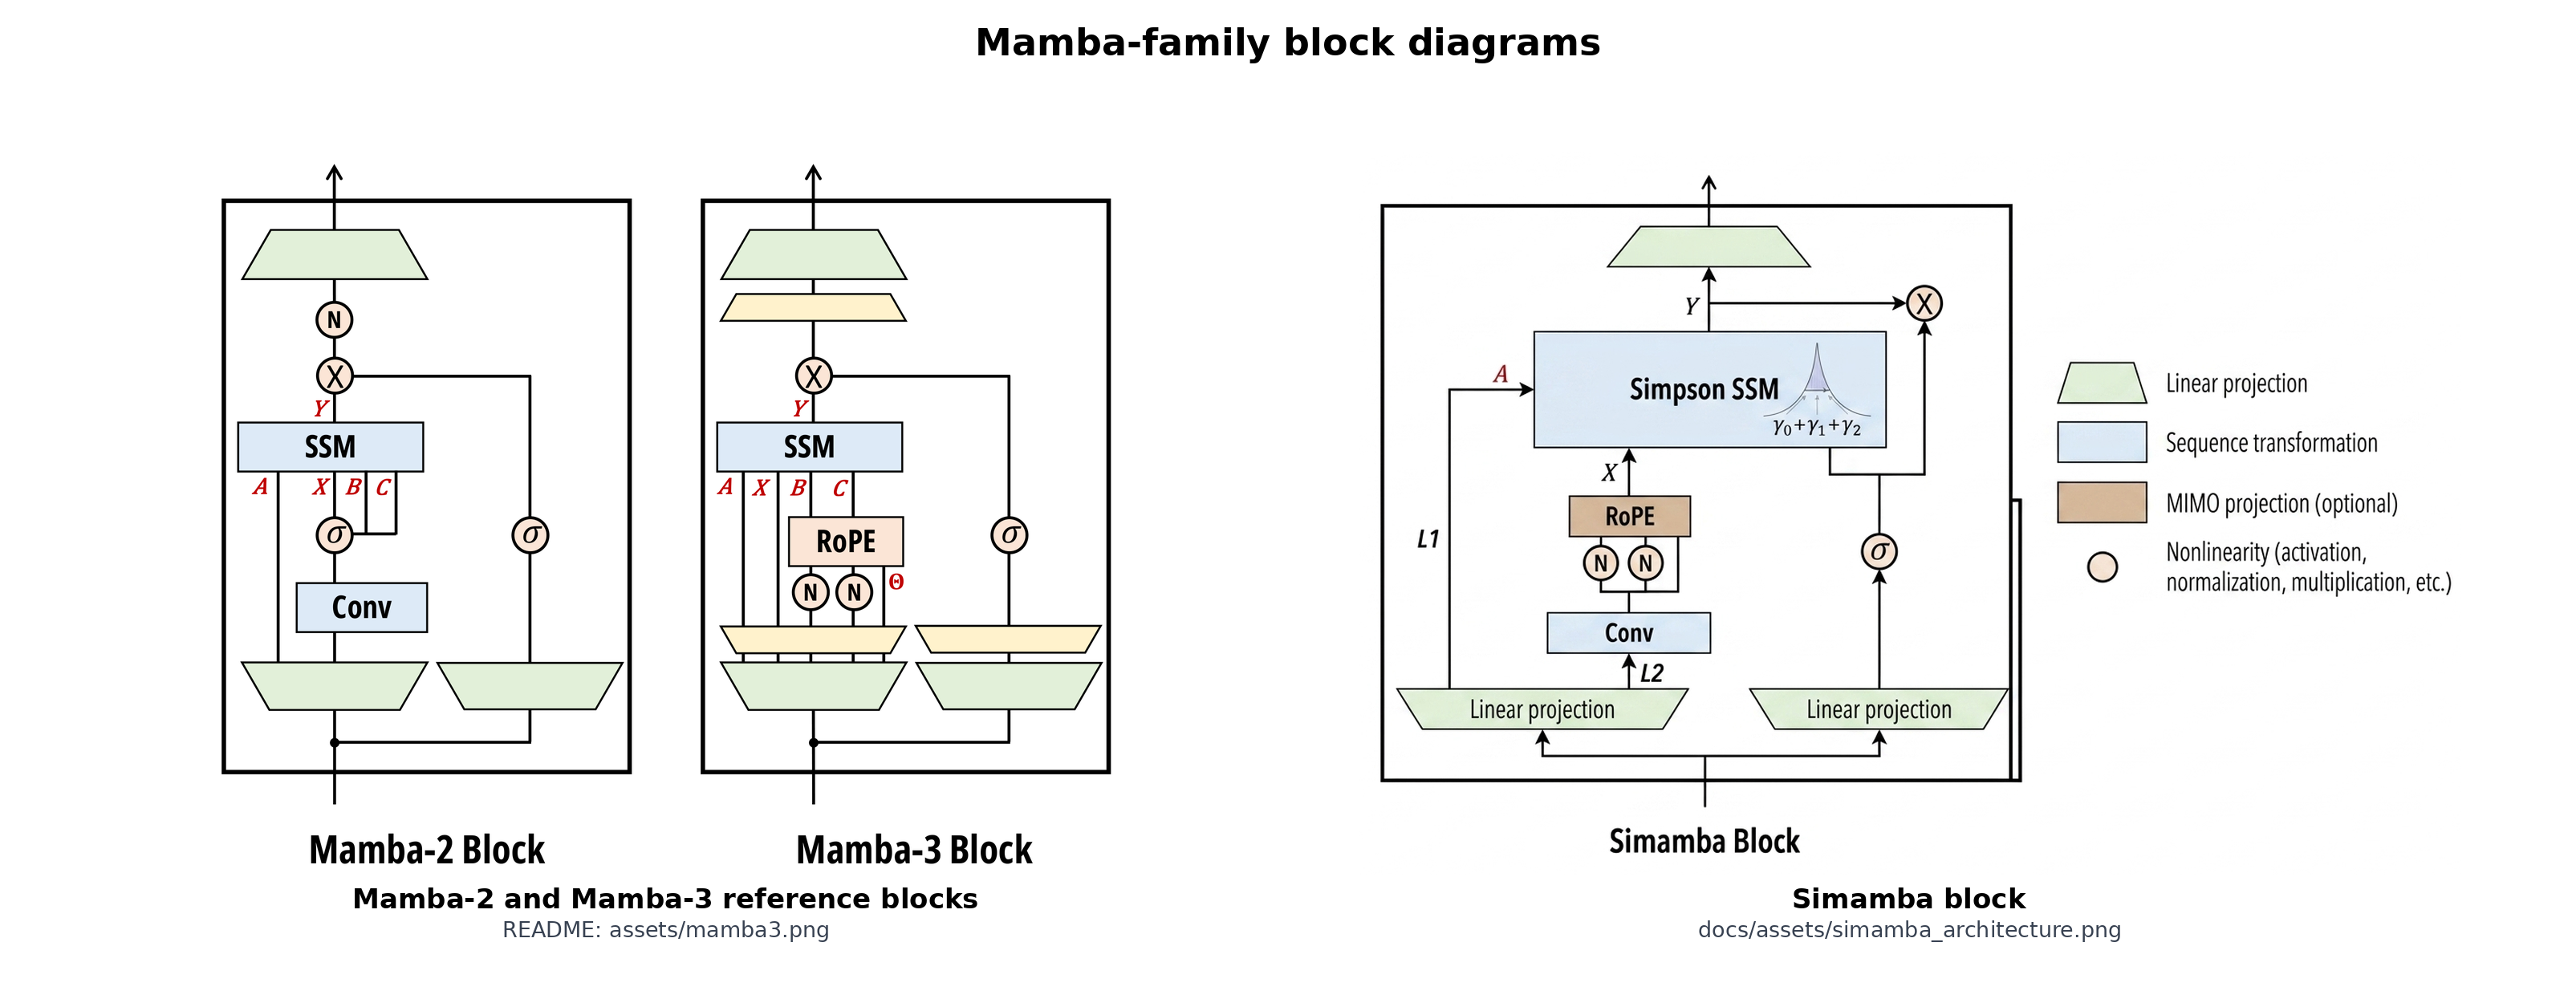
\includegraphics[width=0.98\textwidth]{mamba_family_architecture_comparison.png}
    \caption{Architecture comparison using the README Mamba--2/Mamba--3 block diagram and the added \modelname block diagram. \modelname preserves the Mamba--3-style block skeleton but changes the sequence transformation to a Simpson SSM. The matched trapezoid baseline uses the same projections, biases, rotary state, $D$ skip, and output path; only the SISO state-update coefficients change.}
    \label{fig:arch}
\end{figure*}

\subsection{Matched Trapezoid Baseline}

The comparison baseline is not stock \mambatwo. \mambatwo includes causal local convolution and a different parameterization, so it is not a pure discretization control. We implemented a matched \modelname trapezoid path with the same projection layout as \modelname. Let
\begin{equation}
    \alpha_t=\exp(A_t\Delta_t), \qquad p_t = \sigma(c_t),
\end{equation}
where $c_t$ is the learned trapezoid coefficient logit. The vectorized training form uses a width-2 contribution:
\begin{equation}
    \gamma_t = \Delta_t p_t,\qquad
    s_t = \gamma_t + \Delta_{t+1}(1-p_{t+1}),
\end{equation}
and updates the recurrent state in simplified form as
\begin{equation}
    H_t = \alpha_t H_{t-1} + s_t(v_tk_t^\top).
\end{equation}
The implementation also includes rotary state, $Q/K$ biases, $D$ skip, optional $z$ gate, and fixed boundary handling.

\subsection{Simpson-Style Update}

\modelname{} replaces the trapezoid contribution with a learned width-3 Simpson-like recurrence. Define
\begin{equation}
    \alpha_t = \exp(A_t\Delta_t), \qquad
    \alpha_{t,1/2} = \exp(A_t\Delta_t/2),
\end{equation}
and a bounded learned Simpson correction
\begin{equation}
    s_t = \mathrm{clip}(\sigma(c_t)m_t,0,1),
\end{equation}
where $m_t=1$ unless midpoint control is enabled, in which case $m_t=\sigma(r_t)$ is learned from an additional projection. The coefficients are
\begin{align}
    \gamma_{0,t} &= \frac{\Delta_t}{6}\left(1+\alpha_{t,1/2}(2-\frac{1}{2}s_t)\right),\\
    \gamma_{1,t} &= \frac{\Delta_t}{6}\left(\alpha_t+\alpha_{t,1/2}(2+s_t)\right),\\
    \gamma_{2,t} &= -\frac{\Delta_t}{12}\alpha_{t,1/2}s_t .
\end{align}
The state update is
\begin{equation}
\begin{split}
H_t ={}& \alpha_t H_{t-1}
    + \gamma_{0,t}(v_tk_t^\top)
    + \gamma_{1,t}(v_{t-1}k_{t-1}^\top)\\
    &+ \gamma_{2,t}(v_{t-2}k_{t-2}^\top).
\end{split}
\label{eq:simpson}
\end{equation}
The negative lag-2 term $\gamma_{2,t}$ is the core difference. It is also the most likely source of the noisier gradient norms observed in Fig.~\ref{fig:main_grad}. We therefore added two controls: a coefficient logit offset to initialize $s_t$ closer to zero, and an optional midpoint control to reduce the effective correction.

\section{Implementation}

\subsection{Code Changes}

The main implementation changes are:
\begin{itemize}
    \item \texttt{simamba.py}: \modelname mixer, Simpson/trapezoid switch, coefficient offsets, midpoint control, optional local convolution, and inference cache hooks.
    \item \texttt{simamba\_siso\_combined.py}: reference/vectorized Simpson and matched trapezoid SISO updates.
    \item \texttt{mamba3\_siso\_fwd.py}, \texttt{mamba3\_siso\_bwd.py}, and \texttt{mamba3\_siso\_combined.py}: Triton SISO kernels and the custom PyTorch autograd wrapper for \modelname.
    \item \texttt{train\_simamba\_lm.py}: fixed validation spans, no-replacement epoch sampling, learning-rate decay, nonfinite-step handling, W\&B logging, and checkpoint metadata.
    \item \texttt{prepare\_slimpajama.py}: streaming SlimPajama tokenization into \texttt{uint16} memory maps.
    \item \texttt{eval\_checkpoint\_compression.py}: quantization and pruning perturbation evaluation.
    \item \texttt{generate\_hpml\_paper\_assets.py}: reproducible extraction of local W\&B histories and paper figures.
\end{itemize}

\subsection{PyTorch and Triton Optimizations}

The main HPML implementation work was turning the Simpson SISO recurrence into a trainable GPU operator rather than leaving it as a Python loop. The PyTorch interface is a custom \texttt{torch.autograd.Function} in \texttt{mamba3\_siso\_combined.py}. Its forward path calls a Triton prefill kernel, saves only the tensors needed for differentiation, and exposes the operator as a normal module call inside \texttt{simamba.py}. This let the rest of the model remain ordinary PyTorch: linear projections, optional causal convolution, RMSNorm, AdamW, gradient accumulation, checkpointing, W\&B logging, and optional \texttt{torch.compile} support are handled by the training script. We also keep master parameters in fp32 and use autocast only as an optional activation optimization, because SSM recurrent dynamics were unstable when parameter precision was reduced.

The forward Triton path in \texttt{mamba3\_siso\_fwd.py} computes the SISO recurrent core one program per batch/head tile. It fuses Q/K bias application, rotary-angle use, the Simpson width-3 state update, the $D$ skip term, and optional $z$ gating into one chunked scan over the sequence. The implementation uses explicit pointer arithmetic and stride arguments rather than newer descriptor-only Triton APIs so it can run on the V100 environment used for the experiments. It also includes autotuned stage/warp choices and a fallback step loop for tiny head dimensions that violate Triton's matrix-tile constraints.

The backward pass was the more important correctness optimization. Reusing the original \mambathree trapezoid backward would silently train the wrong model, so \texttt{mamba3\_siso\_bwd.py} implements Simpson-specific reverse-time state propagation. The fused backward kernel computes gradients for $Q$, $K$, $V$, $A\Delta t$, $\Delta t$, the Simpson control, optional midpoint control, Q/K biases, $D$, and recurrent input states while walking chunks in reverse. For the coefficient path, a small Triton step kernel computes per-token dot products against the current SSM adjoint, previous state, and the two lagged $vk^\top$ terms. The wrapper recomputes chunk-start states under \texttt{torch.no\_grad()} instead of storing every intermediate state, which trades extra arithmetic for lower activation memory. A reference/autograd path remains available for edge cases such as stateful inference gradients, and this separation helped debug the original nonfinite-gradient issue.

\subsection{Hugging Face and vLLM Export}

The best \modelname and \mambatwo checkpoints were exported to Hugging Face. The \mambatwo checkpoint was converted to standard \texttt{Mamba2ForCausalLM} layout with \texttt{model\_type=mamba2}, making it natively recognizable by vLLM. \modelname is a custom architecture, so its repository includes \texttt{auto\_map} remote code for \texttt{SimambaModel} and \texttt{SimambaForCausalLM}; vLLM can serve it through the Transformers backend with \texttt{--trust-remote-code --model-impl transformers}. This preserves the architecture rather than pretending \modelname is \mambatwo.

\section{Data and Training Setup}

\subsection{Dataset Preparation}

We use SlimPajama \cite{slimpajama}, streamed from Hugging Face with the GPT-NeoX tokenizer. Documents are tokenized without extra special tokens, an EOS token is appended, and token IDs are stored as \texttt{uint16} memory-mapped arrays because the vocabulary fits in 16 bits. The primary dataset contains 500M train tokens and 50M validation tokens:
\begin{center}
\begin{tabular}{@{}lrr@{}}
\toprule
Split & Tokens & Documents\\
\midrule
Train & 500M & 691,532\\
Validation & 50M & 49,451\\
\bottomrule
\end{tabular}
\end{center}
The memory maps are stored under \path{data/slimpajama_500m_50m/}. We also prepared a 100M/10M split and tiny smoke-test subsets, but the main comparisons use 500M/50M or 50M-token budgets from the same prepared data.

\subsection{Hardware and Runtime}

The original target was four NVIDIA RTX A6000 GPUs on a Slurm cluster. That environment was unreliable, so the final experiments were run on a single NVIDIA Tesla V100-SXM2 16GB. This shaped the experimental design: we used a 10M-parameter model for controlled ablations, sequence length 128, global batch size 64, micro-batch size 8, and gradient accumulation over 8 microsteps. The largest useful 50M-parameter attempt was dominated by compilation/runtime pressure, so it was not used as the scientific comparison.

\subsection{Deep Learning Techniques}

The training stack used the following techniques:
\begin{itemize}
    \item AdamW with weight decay for language-model pretraining \cite{adamw}.
    \item Linear warmup followed by cosine decay. The early unstable runs used an over-aggressive schedule; adding decay and reducing peak learning rate was essential.
    \item Gradient accumulation to fit the effective global batch on a 16GB V100.
    \item Gradient clipping at 1.0, with both pre-clip and post-clip norms logged. Clipping is a guardrail, not a cure for divergence.
    \item fp32 parameter storage and fp32 final comparisons. This follows the Mamba observation that SSM recurrent dynamics are sensitive to low-precision parameter storage \cite{mamba}.
    \item Fixed validation sampling: every run evaluates the same validation spans, which makes curves comparable.
    \item No-replacement epoch sampling: training draws shuffled non-overlapping token blocks rather than sampling with replacement.
    \item Nonfinite-step detection, checkpoint manifests, W\&B run IDs, and resume metadata for long-run reliability.
    \item DDP-ready initialization: the script can initialize distributed data parallel training, but the reported final experiments use world size 1 on the V100.
\end{itemize}

\section{Experiments and Results}

All learning-curve figures in this section are exported from locally persisted W\&B/training histories. The W\&B API key was not present in the report-generation shell, so the script reconstructs the curves from the synchronized local W\&B output logs and JSON metric records.

\subsection{Initial Instability}

The first failure mode was exploding or nonfinite gradients before warmup completed. The loss appeared to plateau because clipping forced updates to a bounded norm, but gradient-health logs later showed nonfinite parameters/gradients. Fig.~\ref{fig:instability} shows the representative unstable run: the pre-clip gradient norm remains large while the learning rate is still tiny, and the job terminates at the first nonfinite detection.

\begin{figure}[t]
    \centering
    
\includegraphics[width=\columnwidth]{wandb_initial_instability.png}
    \caption{Initial unstable run. Gradient clipping held the post-clip update at 1.0, but the pre-clip norm stayed large and a nonfinite gradient was detected at step 159.}
    \label{fig:instability}
\end{figure}

The fixes were fp32 parameters, cosine decay after warmup, lower peak learning rates for larger runs, nonfinite skip/abort handling, and clearer W\&B/checkpoint resume metadata. These changes made the controlled fp32 runs complete with zero nonfinite skips.

\subsection{Main 500M-Token Comparison}

The primary comparison trains 10M-parameter models on one pass over 500M tokens, then continues the main variants for a second pass when useful. Model dimensions are $d_{\mathrm{model}}=160$, 8 layers, $d_{\mathrm{state}}=64$, head dimension 32, sequence length 128, and tied input/output embeddings.

\begin{table}[t]
\caption{Main 500M-token language-model comparison.}
\label{tab:main}
\centering
\footnotesize
\begin{tabular}{@{}lrrrr@{}}
\toprule
Model & Best val. & Step & Last val. & Last train\\
\midrule
\mambatwo & 4.8625 & 122k & 4.8625 & 4.2041\\
\modelname{} Simpson & 4.9319 & 89k & 4.9671 & 4.3852\\
\modelname{} Simpson+midpoint & 4.9178 & 71k & 4.9889 & 4.3816\\
\modelname{} trapezoid & 4.9326 & 61k & 4.9326 & 4.4823\\
\bottomrule
\end{tabular}
\end{table}

\begin{figure}[t]
    \centering
    
\includegraphics[width=\columnwidth]{wandb_main_500m_val_loss.png}
    \caption{Fixed validation loss on the 500M-token comparison. \mambatwo continues improving through the second pass; Simpson variants begin to degrade on validation after their best checkpoints.}
    \label{fig:main_val}
\end{figure}

\begin{figure}[t]
    \centering
    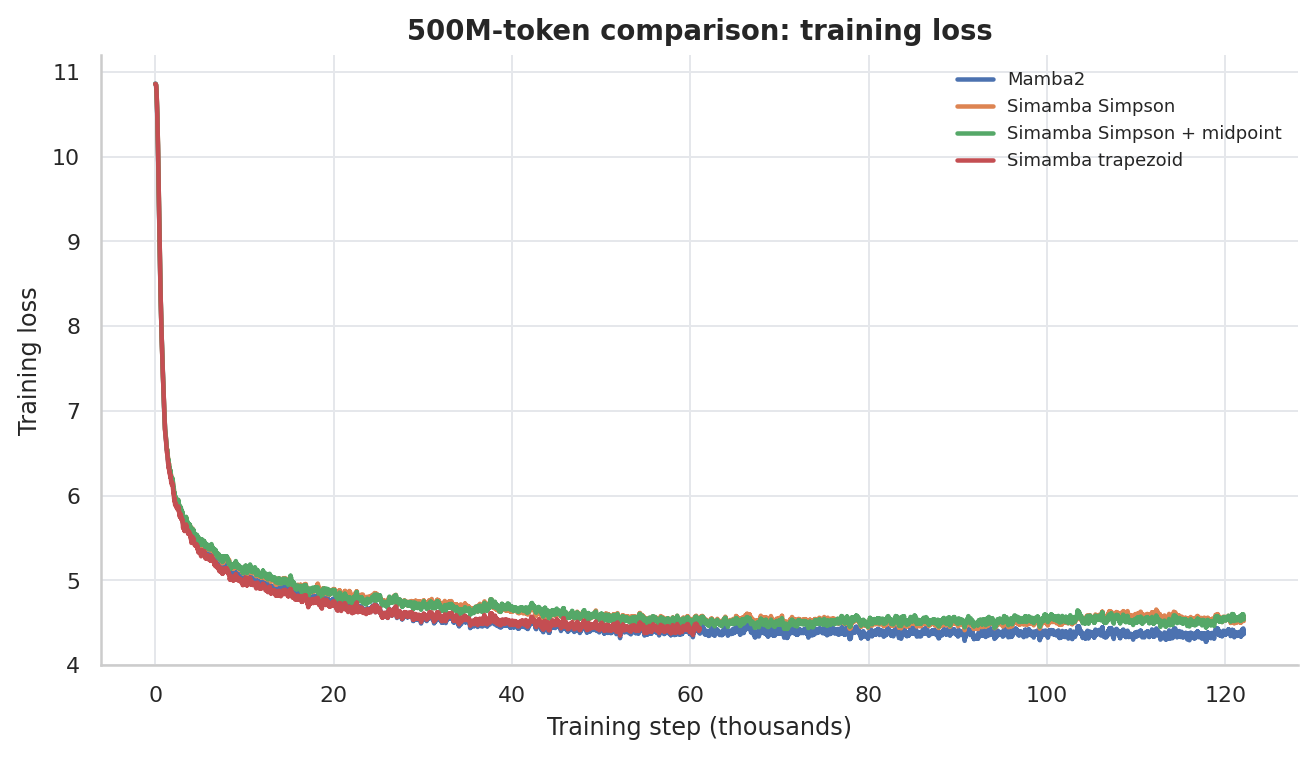
\includegraphics[width=\columnwidth]{wandb_main_500m_train_loss.png}
    \caption{Smoothed training loss for the 500M-token comparison. All models learn the training distribution, so the validation gap is not caused by a broken data path.}
    \label{fig:main_train}
\end{figure}

\begin{figure}[t]
    \centering
    
\includegraphics[width=\columnwidth]{wandb_main_500m_grad_norm.png}
    \caption{Smoothed pre-clip gradient norm. The Simpson variants show larger tail gradient norms than \mambatwo and the matched trapezoid run, consistent with harder optimization.}
    \label{fig:main_grad}
\end{figure}

The validation curves in Fig.~\ref{fig:main_val} are the strongest evidence against the current Simpson formulation. \mambatwo is the best overall model, but it is not a pure discretization baseline. More importantly, the matched \modelname trapezoid baseline is competitive with and slightly better than default Simpson, while Simpson+midpoint has a better best checkpoint but worse final validation.

\subsection{Matched 50M-Token Discretization Ablation}

To reduce runtime and isolate the discretization, we ran a 50M-token matched ablation with identical model size, data, batch size, seed, and schedule. Table~\ref{tab:ablation50} and Fig.~\ref{fig:ablation50} show that lowering the initial Simpson correction helps, but not enough to beat trapezoid.

\begin{table}[t]
\caption{50M-token matched discretization ablation.}
\label{tab:ablation50}
\centering
\begin{tabular}{lrrr}
\toprule
Variant & Best/final val. & Last train & Skips\\
\midrule
Trapezoid & 5.8195 & 5.6111 & 0\\
Simpson default & 5.9178 & 5.7161 & 0\\
Simpson low-control & 5.8929 & 5.6995 & 0\\
\bottomrule
\end{tabular}
\end{table}

\begin{figure}[t]
    \centering
    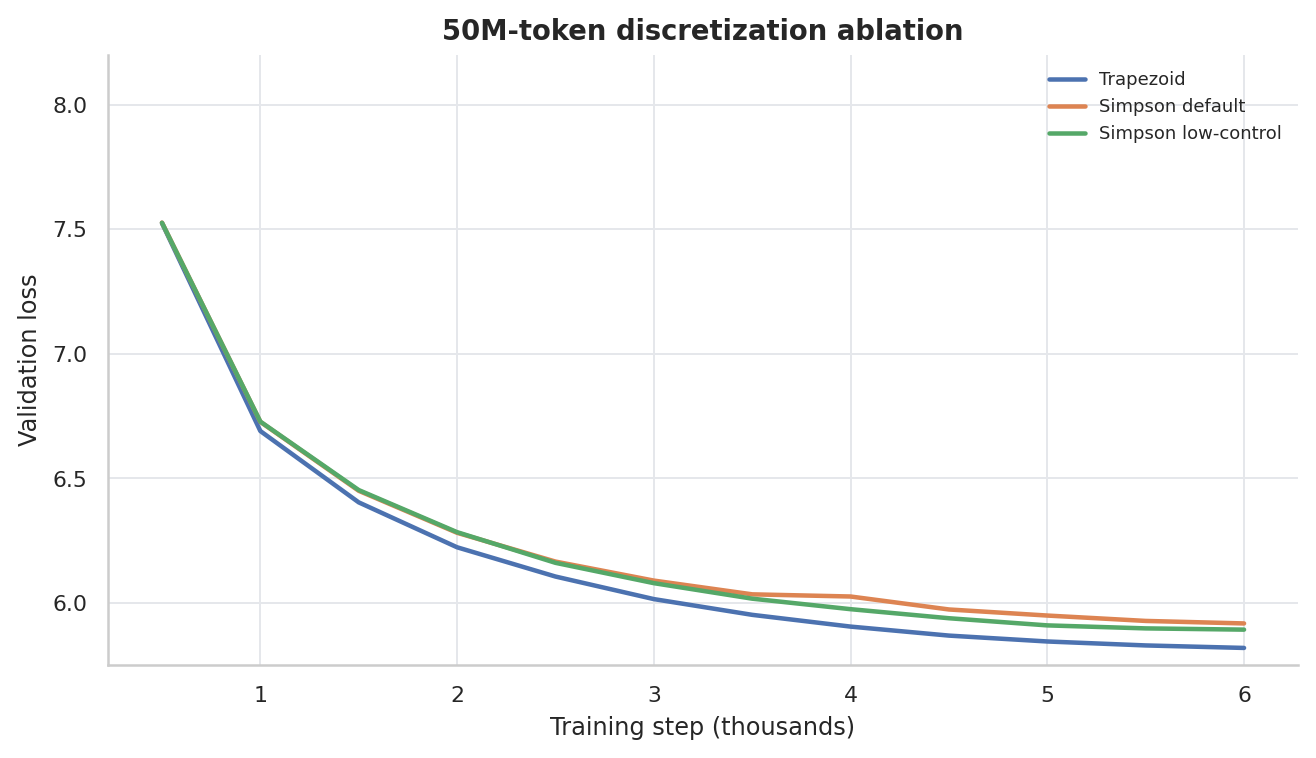
\includegraphics[width=\columnwidth]{wandb_50m_discretization_val_loss.png}
    \caption{50M-token discretization ablation. The low-control initialization improves Simpson, but the matched trapezoid update remains ahead.}
    \label{fig:ablation50}
\end{figure}

\subsection{Local-Convolution Confound}

\mambatwo includes a depthwise causal convolution over the $x/B/C$ stream before the SSM update. \modelname initially did not. This matters: removing or shrinking \mambatwo's convolution hurts quality, as shown in Table~\ref{tab:local}. We therefore added \texttt{--simamba-d-conv 4} to give \modelname the same local-mixing control.

\begin{table}[t]
\caption{Local-mixing controls on 50M tokens.}
\label{tab:local}
\centering
\begin{tabular}{lrr}
\toprule
Variant & Best/final val. & Last train\\
\midrule
\mambatwo{} $d_{\mathrm{conv}}=2$ & 5.8425 & 5.6268\\
\mambatwo{} $d_{\mathrm{conv}}=1$ & 5.9001 & 5.6958\\
\modelname{} local-conv trapezoid & 5.8469 & 5.6309\\
\modelname{} local-conv Simpson low-control & 5.8793 & 5.6701\\
\modelname{} local-conv Simpson & 5.8890 & 5.6759\\
\bottomrule
\end{tabular}
\end{table}

\begin{figure}[t]
    \centering
    
\includegraphics[width=\columnwidth]{wandb_localmix_val_loss.png}
    \caption{Local-mixing controls. Adding Mamba2-style local mixing narrows the gap for Simpson, but local-conv trapezoid is still better at this budget.}
    \label{fig:localmix}
\end{figure}

This experiment is important because it prevents a misleading \mambatwo-vs-\modelname conclusion. Some of \mambatwo's advantage comes from local mixing, not only from its state discretization. After matching that mechanism, Simpson still trails the matched trapezoid update.

\subsection{Throughput and Kernel Benchmarking}

Training throughput on the V100 is shown in Fig.~\ref{fig:throughput}. The non-local Simpson variants are slower than \mambatwo and trapezoid in the 500M runs, while the local-conv 50M runs are closer but still behind the fastest baselines.

\begin{figure}[t]
    \centering
    
\includegraphics[width=\columnwidth]{wandb_training_throughput.png}
    \caption{Median tail training throughput on the V100, computed from the last 100 logged W\&B points for each run.}
    \label{fig:throughput}
\end{figure}

The repository SISO benchmark further separates prefill and decode. The current \modelname prefill path is much slower than the \mambathree fused kernel path: 776.9$\times$ slower in the B1/P128/G64 case and 410.7$\times$ slower in B4/P1024/G256. Decode-step latency is much closer, about 1.08$\times$ slower. Memory is comparable at decode and can be lower for \modelname prefill in the B4/P1024 case, but the latency gap dominates.

\begin{figure}[t]
    \centering
    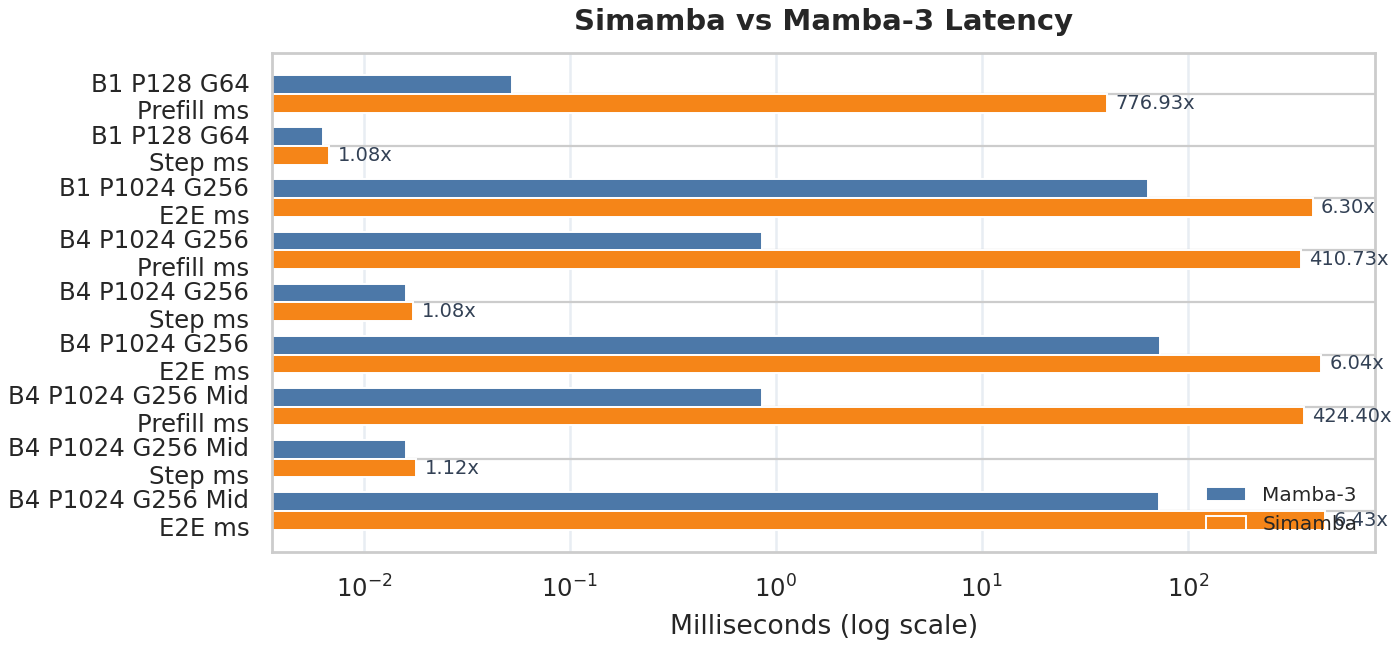
\includegraphics[width=\columnwidth]{simamba_latency.png}
    \caption{Repository SISO benchmark latency. \modelname decode overhead is small, but the prefill implementation is not competitive without fused-kernel work.}
    \label{fig:bench_latency}
\end{figure}

\begin{figure}[t]
    \centering
    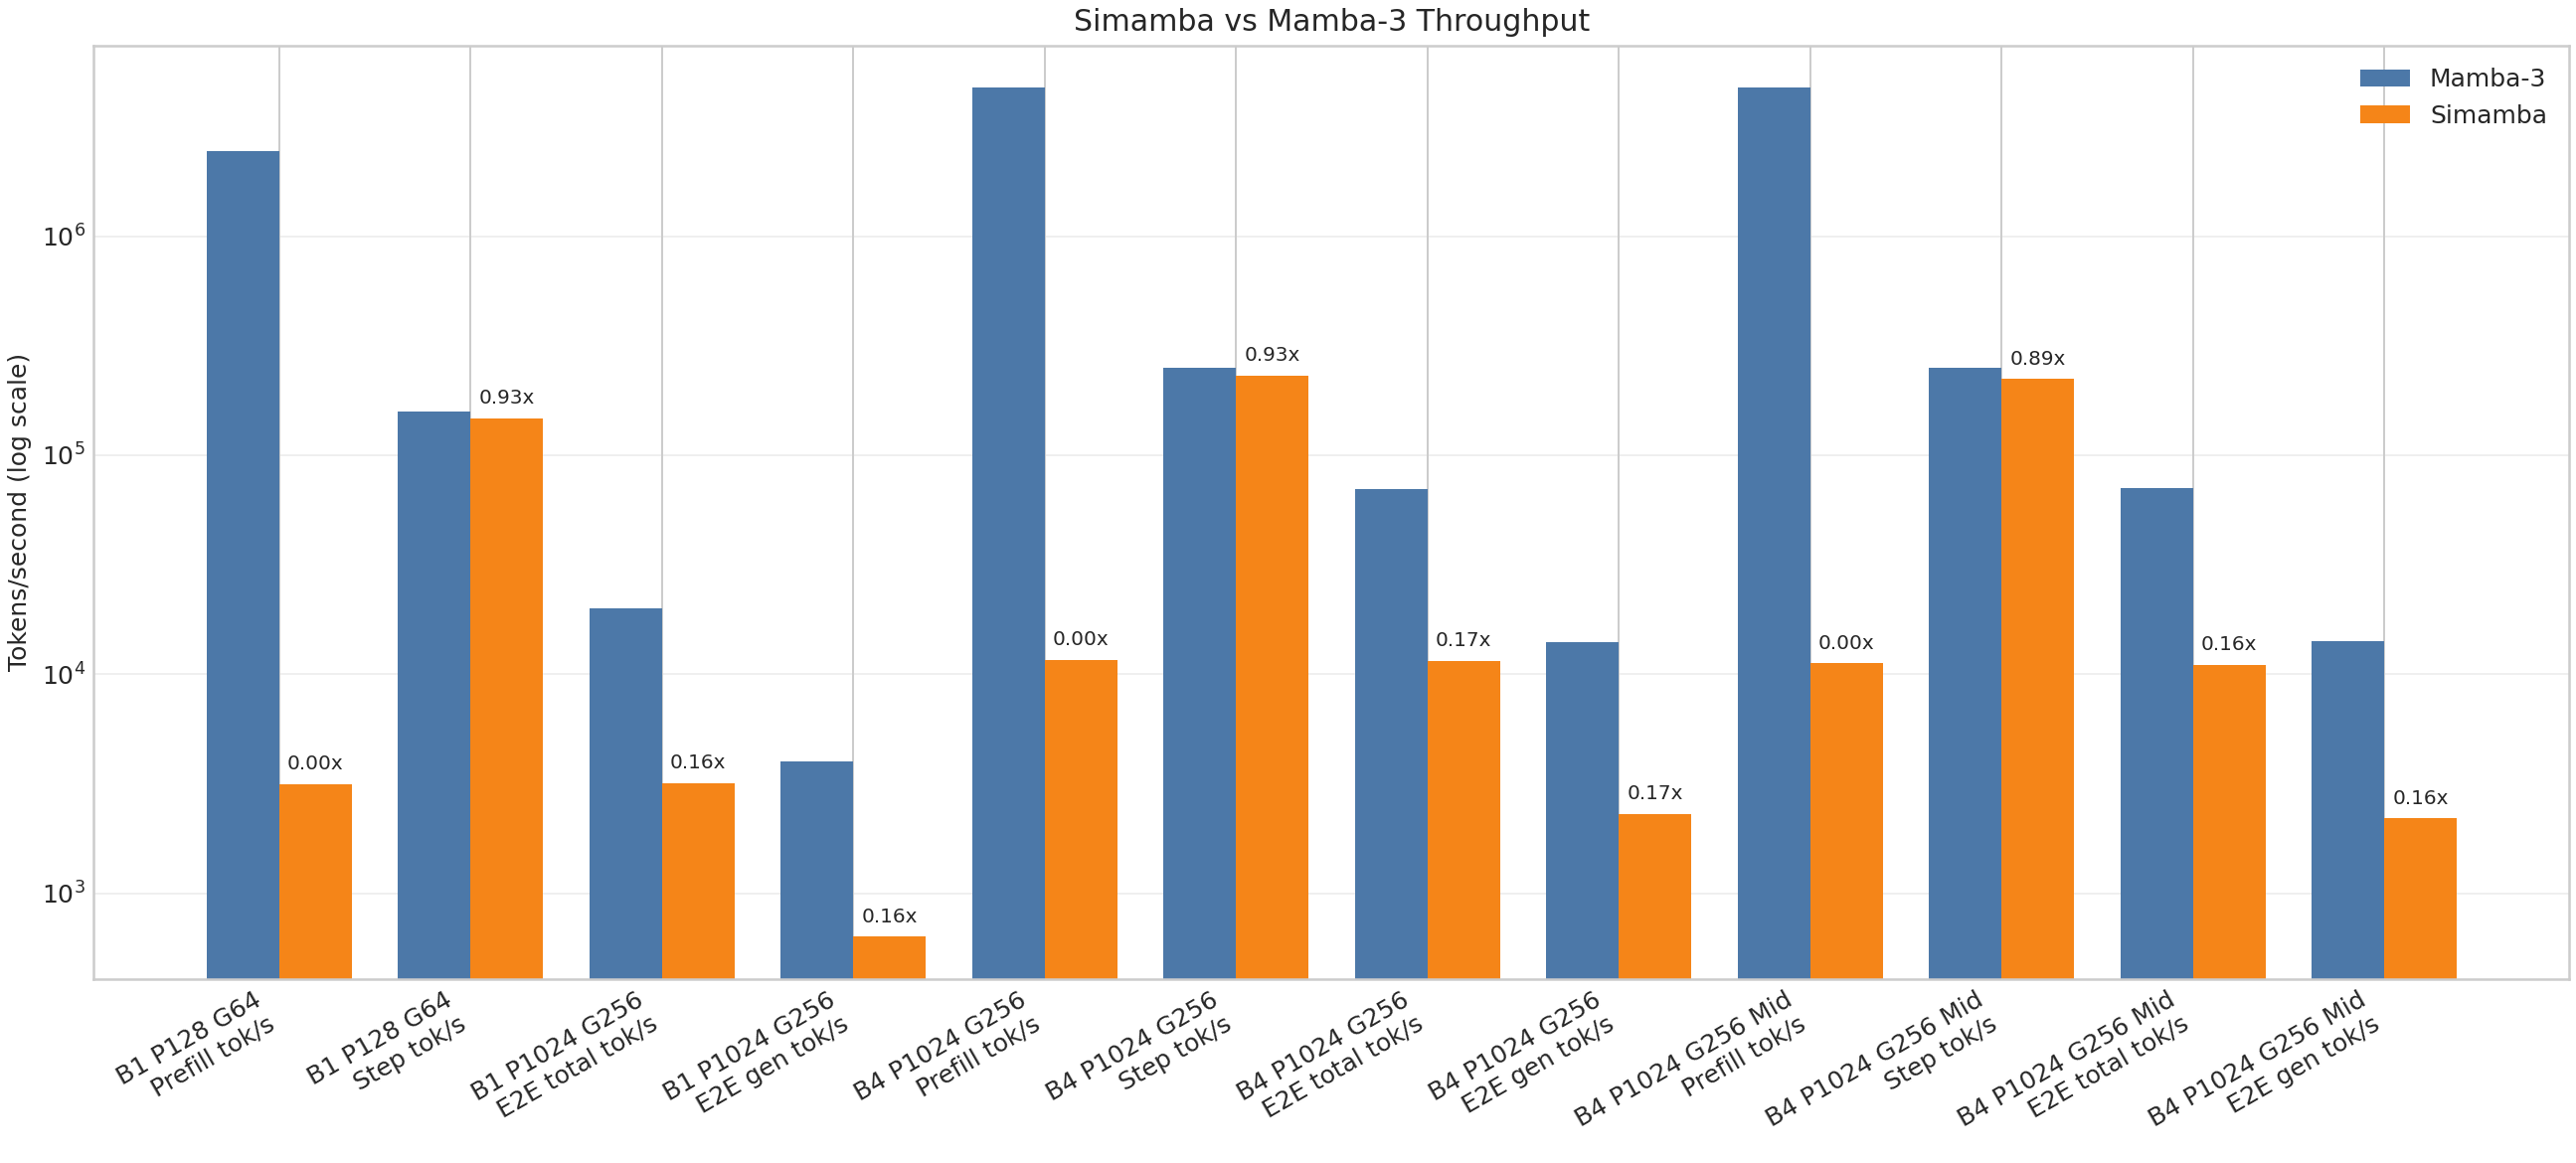
\includegraphics[width=\columnwidth]{simamba_throughput.png}
    \caption{Repository SISO benchmark throughput. The current prefill gap is a systems bottleneck independent of validation loss.}
    \label{fig:bench_throughput}
\end{figure}

\subsection{Synthetic State Tracking}

We also added a small synthetic classifier harness for algorithmic state-tracking tasks such as parity and modular sum. The motivation was that Simpson-style recurrences might help tasks with explicit state evolution even if the language-model result is negative. The recorded modular-sum \modelname Simpson run did not produce a useful positive result: final metrics were approximately loss 2.7811 and accuracy 0.0508 at length 128, and loss 2.7805 and accuracy 0.0542 at length 256. These tasks remain diagnostics rather than evidence for the main claim.

\subsection{Compression and Pruning}

Compression was evaluated as a side experiment using non-destructive weight perturbations on fixed validation spans. Row-wise int8 quantize-dequantize is nearly lossless for all three checkpoints, while int4 and unstructured pruning beyond 10\% cause substantial degradation.

\begin{figure}[t]
    \centering
    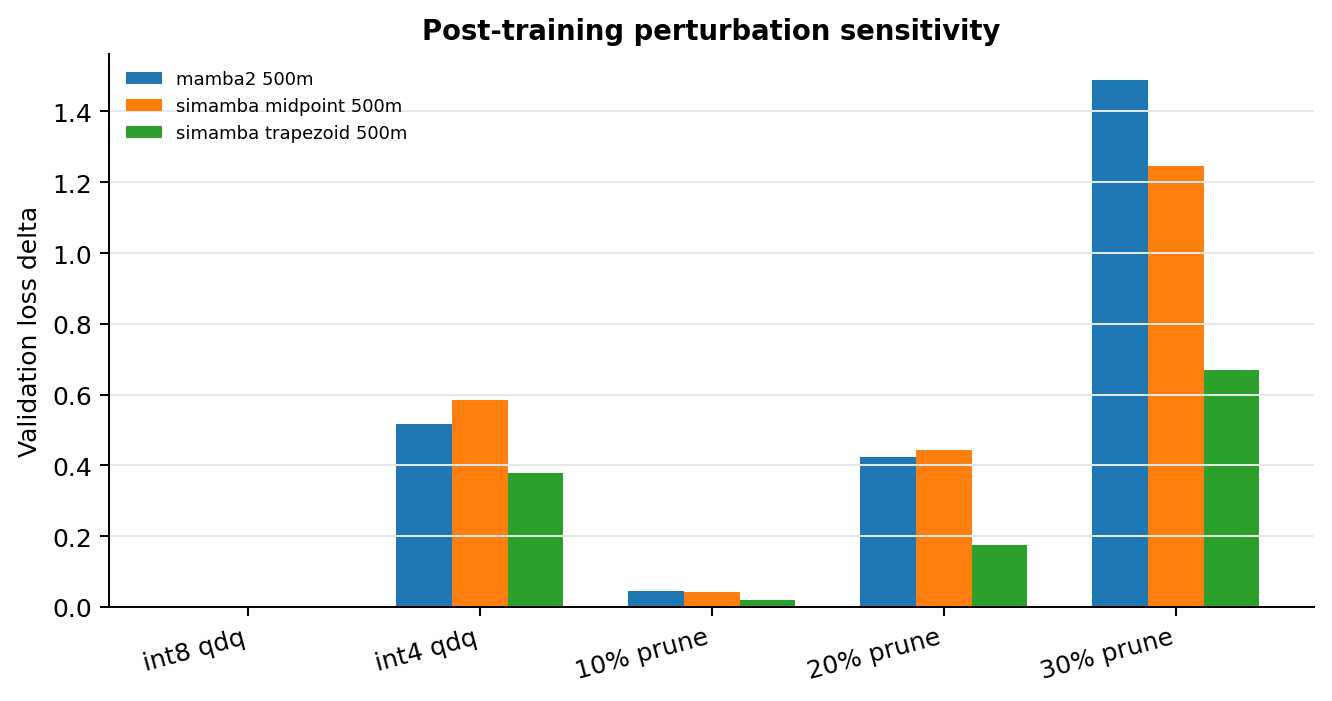
\includegraphics[width=\columnwidth]{compression_loss_delta.png}
    \caption{Validation loss delta after post-training perturbations. Int8 row-wise quantize-dequantize is nearly lossless; int4 and larger pruning ratios require finetuning or better kernels.}
    \label{fig:compression}
\end{figure}

\begin{table}[t]
\caption{Compression perturbation loss deltas.}
\label{tab:compression}
\centering
\begin{tabular}{lrrrr}
\toprule
Checkpoint & int8 & int4 & 10\% prune & 30\% prune\\
\midrule
\mambatwo{} best & +0.0019 & +0.5181 & +0.0457 & +1.4881\\
\modelname{} midpoint & +0.0014 & +0.5846 & +0.0433 & +1.2446\\
\modelname{} trapezoid & +0.0013 & +0.3771 & +0.0207 & +0.6680\\
\bottomrule
\end{tabular}
\end{table}

\subsection{Qualified Positive Results}

Although the headline language-model result is negative, three bounded positive results are worth recording. First, in the 500M-token comparison, \modelname{} Simpson+midpoint reaches a better best checkpoint than the matched \modelname{} trapezoid baseline (4.9178 vs. 4.9326), although it does not hold that advantage at the final validation point. Second, after adding matched local convolution, \modelname{} Simpson low-control beats the weakened \mambatwo{} $d_{\mathrm{conv}}=1$ control (5.8793 vs. 5.9001), which shows that part of the initial gap was a local-mixing confound. Third, the compression perturbations show that \modelname{} checkpoints are competitive in some post-training robustness settings: the midpoint checkpoint has a slightly smaller int8 loss delta than \mambatwo{} (+0.0014 vs. +0.0019), and the trapezoid checkpoint has lower int4 and pruning deltas. These are not enough to claim a \modelname{} architecture win, but they identify controlled settings where the implementation is competitive and worth improving.

\subsection{Overall Result}

The result summary is direct: the current Simpson recurrence is trainable but not superior. The strongest \modelname Simpson checkpoint is the midpoint-control model at 4.9178 validation loss, but the best overall language model is \mambatwo at 4.8625, and the matched trapezoid controls remain at least competitive across budgets.

\section{Discussion}

\subsection{Why Simpson Underperformed}

The results suggest three interacting causes. First, Simpson's higher-order quadrature rationale assumes smooth forcing terms, but token-level language inputs are discontinuous and highly data dependent. Second, the learned negative lag-2 coefficient in (\ref{eq:simpson}) can produce cancellation and noisier gradients, especially early in training before the model has learned stable coefficients. Third, \mambatwo's local convolution is a major architectural confound; once we matched local mixing, Simpson improved but still did not beat trapezoid.

This does not prove that Simpson-style discretization is impossible for SSMs. It shows that the current direct parameterization is not enough. A better design may need a constrained positive decomposition, an annealed correction schedule, or a trust-region style bound on the lag-2 term.

\subsection{Systems Lessons}

The project also exposed a systems gap. Even if Simpson quality were better, the current prefill implementation would not be practical in production. The decode step is close to \mambathree, but prefill needs a fused kernel that combines projection layout, local convolution, recurrence, and output projection without Python-level loops or excessive memory traffic. The V100 also lacks some newer Triton functionality used by the \mambathree kernels, so a portable fallback path is needed for older GPUs.

\section{Future Work}

The most important next steps are:
\begin{itemize}
    \item Reparameterize the Simpson correction so the negative lag-2 term cannot dominate early training.
    \item Anneal the Simpson coefficient from zero after the model has learned a stable trapezoid-like recurrence.
    \item Build a fused local-conv \modelname kernel and a V100-compatible benchmark fallback.
    \item Run multi-seed 50M-token comparisons only after a single-seed Simpson variant beats the matched trapezoid baseline.
    \item Evaluate on longer context lengths, where higher-order state updates may have a better chance to matter.
    \item Add finetuning-aware int4 and pruning experiments rather than one-shot perturbations.
    \item Integrate the custom \modelname remote-code path more deeply into vLLM if the architecture becomes quality-positive.
\end{itemize}

\section{Conclusion}

We implemented and evaluated \modelname, a Simpson-style SISO discretization for \mambathree-inspired language models. The engineering outcome is strong: the data pipeline, training loop, validation protocol, checkpointing, W\&B logging, compression evaluation, benchmarking, and model export paths are now reproducible on a single V100. The scientific outcome is negative but informative: the current Simpson recurrence does not beat \mambatwo or the matched trapezoid baseline, and the evidence points to optimization difficulty from the negative lag-2 correction. Future work should treat Simpson as a constrained or annealed correction to a stable trapezoid recurrence rather than as an unconstrained replacement.

\section*{Artifact Availability}

{\raggedright
The best checkpoints are available as Hugging Face repositories \path{soumil1/simamba-midpoint-10m-slimpajama-500m} and \path{soumil1/mamba2-10m-slimpajama-500m}. The local paper assets are generated by \texttt{scripts/generate\_hpml\_paper\_assets.py}.
\par}

\begin{thebibliography}{00}
\bibitem{mamba}
A. Gu and T. Dao, ``Mamba: Linear-time sequence modeling with selective state spaces,'' arXiv:2312.00752, 2023.

\bibitem{mamba2}
T. Dao and A. Gu, ``Transformers are SSMs: Generalized models and efficient algorithms through structured state space duality,'' in \textit{Proc. International Conference on Machine Learning}, 2024.

\bibitem{mamba3}
A. Lahoti, K. Y. Li, B. Chen, C. Wang, A. Bick, J. Z. Kolter, T. Dao, and A. Gu, ``Mamba-3: Improved sequence modeling using state space principles,'' arXiv:2603.15569, 2026.

\bibitem{flashattention}
T. Dao, D. Y. Fu, S. Ermon, A. Rudra, and C. Re, ``FlashAttention: Fast and memory-efficient exact attention with IO-awareness,'' in \textit{Advances in Neural Information Processing Systems}, 2022.

\bibitem{adamw}
I. Loshchilov and F. Hutter, ``Decoupled weight decay regularization,'' in \textit{Proc. International Conference on Learning Representations}, 2019.

\bibitem{slimpajama}
Cerebras Systems, ``SlimPajama: A 627B token cleaned and deduplicated version of RedPajama,'' Hugging Face dataset, 2023. [Online]. Available: \url{https://huggingface.co/datasets/cerebras/SlimPajama-627B}

\bibitem{gptneox}
S. Black, S. Biderman, E. Hallahan, Q. Anthony, L. Gao, L. Golding, H. He, C. Leahy, K. McDonell, J. Phang, M. Pieler, U. S. Prashanth, S. Purohit, L. Reynolds, J. Tow, B. Wang, and S. Weinbach, ``GPT-NeoX-20B: An open-source autoregressive language model,'' arXiv:2204.06745, 2022.

\bibitem{vllm}
W. Kwon, Z. Li, S. Zhuang, Y. Sheng, L. Zheng, C. H. Yu, J. Gonzalez, H. Zhang, and I. Stoica, ``Efficient memory management for large language model serving with PagedAttention,'' in \textit{Proc. ACM Symposium on Operating Systems Principles}, 2023.
\end{thebibliography}

\end{document}
